% Source: graduate-coursework/Research/Intro_to_Agents/handouts/Part7_Parallelization.tex

\documentclass[border=4pt]{standalone}
\usepackage{amsmath,amssymb,amsfonts}
\usepackage[T1]{fontenc}
\usepackage{graphicx}
\usepackage{lmodern}
\usepackage{tikz}
\usepackage{xcolor}
\usetikzlibrary{shapes.geometric, arrows.meta, positioning, calc, fit, backgrounds, matrix, decorations.pathreplacing}

\definecolor{UofSCGarnet}{HTML}{73000a}
\definecolor{UofSCBlack}{HTML}{000000}
\definecolor{UofSCWhite}{HTML}{ffffff}
\definecolor{UofSCRose}{HTML}{CC2E40}
\definecolor{UofSCAtlantic}{HTML}{466A9F}
\definecolor{UofSCCongaree}{HTML}{1F414D}
\definecolor{UofSCHorseshoe}{HTML}{65780B}
\definecolor{UofSCGrass}{HTML}{CED318}
\definecolor{UofSCHoneycomb}{HTML}{A49137}
\definecolor{UofSC90Black}{HTML}{363636}
\definecolor{UofSC70Black}{HTML}{5C5C5C}
\definecolor{UofSC50Black}{HTML}{A2A2A2}
\definecolor{UofSCWarmGrey}{HTML}{676156}
\definecolor{UofSCSandstorm}{HTML}{FFF2E3}
\definecolor{UofSCDarkGarnet}{HTML}{570008}
\definecolor{UofSCAzalea}{HTML}{844247}

\tikzset{
    % Node styles - all with sharp corners
    agentbox/.style={
        rectangle,
        draw=UofSCGarnet,
        fill=UofSCSandstorm,
        thick,
        minimum width=2cm,
        minimum height=0.8cm,
        text centered,
        font=\footnotesize
    },
    processbox/.style={
        rectangle,
        draw=UofSCAtlantic,
        fill=UofSCWhite,
        thick,
        minimum width=2.5cm,
        minimum height=0.7cm,
        text centered,
        font=\footnotesize
    },
    syncbox/.style={
        rectangle,
        draw=UofSCCongaree,
        fill=UofSCCongaree!20,
        thick,
        minimum width=3cm,
        minimum height=0.5cm,
        text centered,
        font=\footnotesize\bfseries
    },
    resultbox/.style={
        rectangle,
        draw=UofSCHorseshoe,
        fill=UofSCGrass!30,
        thick,
        minimum width=2cm,
        minimum height=0.7cm,
        text centered,
        font=\footnotesize
    },
    % Arrow styles
    myarrow/.style={
        ->,
        >=Stealth,
        thick,
        UofSCBlack
    },
    dashedarrow/.style={
        ->,
        >=Stealth,
        thick,
        dashed,
        UofSC70Black
    },
    % Timeline styles
    timeline/.style={
        draw=UofSCBlack,
        thick,
        ->,
        >=Stealth
    },
    timeblock/.style={
        rectangle,
        draw=none,
        minimum height=0.5cm,
        text centered,
        font=\tiny
    }
}

\begin{document}
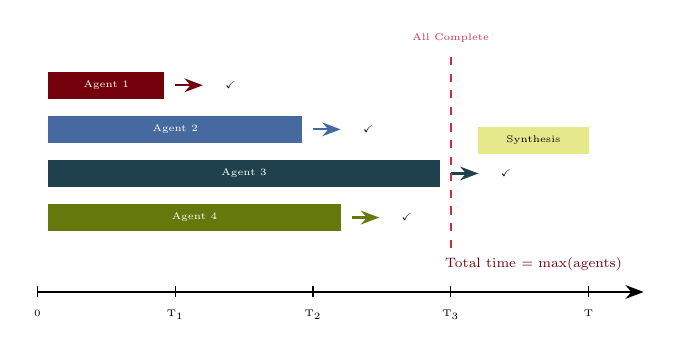
\begin{tikzpicture}[scale=0.7, transform shape]
            % Timeline axis
            \draw[timeline] (0,0) -- (11,0);
            \foreach \x/\l in {0/0,2.5/T$_1$,5/T$_2$,7.5/T$_3$,10/T} {
                \draw (\x,-0.1) -- (\x,0.1);
                \node[font=\tiny,below] at (\x,-0.2) {\l};
            }

            % Agent 1 - fast
            \fill[UofSCGarnet] (0.2,3.5) rectangle (2.3,4);
            \node[font=\tiny,white] at (1.25,3.75) {Agent 1};
            \draw[myarrow,UofSCGarnet] (2.5,3.75) -- (3,3.75);
            \node[font=\tiny] at (3.5,3.75) {\checkmark};

            % Agent 2 - medium
            \fill[UofSCAtlantic] (0.2,2.7) rectangle (4.8,3.2);
            \node[font=\tiny,white] at (2.5,2.95) {Agent 2};
            \draw[myarrow,UofSCAtlantic] (5,2.95) -- (5.5,2.95);
            \node[font=\tiny] at (6,2.95) {\checkmark};

            % Agent 3 - slow
            \fill[UofSCCongaree] (0.2,1.9) rectangle (7.3,2.4);
            \node[font=\tiny,white] at (3.75,2.15) {Agent 3};
            \draw[myarrow,UofSCCongaree] (7.5,2.15) -- (8,2.15);
            \node[font=\tiny] at (8.5,2.15) {\checkmark};

            % Agent 4 - medium
            \fill[UofSCHorseshoe] (0.2,1.1) rectangle (5.5,1.6);
            \node[font=\tiny,white] at (2.85,1.35) {Agent 4};
            \draw[myarrow,UofSCHorseshoe] (5.7,1.35) -- (6.2,1.35);
            \node[font=\tiny] at (6.7,1.35) {\checkmark};

            % Completion line
            \draw[thick,dashed,UofSCRose] (7.5,0.8) -- (7.5,4.3);
            \node[font=\tiny,UofSCRose] at (7.5,4.6) {All Complete};

            % Synthesis
            \fill[UofSCGrass!50] (8,2.5) rectangle (10,3);
            \node[font=\tiny] at (9,2.75) {Synthesis};

            % Annotations
            \node[font=\scriptsize,UofSCGarnet] at (9,0.5) {Total time = max(agents)};
        \end{tikzpicture}
\end{document}
